% !TeX encoding = UTF-8
% !TeX spellcheck = en_US
\documentclass[a4paper,11pt]{article}
\usepackage[hmargin=3cm,vmargin=4cm,centering,foot=1.5cm,includefoot]{geometry}
\usepackage[T1]{fontenc}
\usepackage[utf8]{inputenc}
\usepackage[english]{babel}
\usepackage{palatino}
\usepackage[scaled]{beramono}
\usepackage{eulervm}
\usepackage{graphicx}
\usepackage[pdfhighlight=/O,linkcolor=blue]{hyperref}
\hypersetup{
	pdfborder={0 0 0},
	pdfauthor={Federico Soave},
	pdftitle={Game of Life - SPM project report},
	pdfkeywords={},
	pdfcreator={},
	pdfproducer={},
}
\usepackage{listings}
\usepackage{array}
\setlength{\extrarowheight}{2pt}
\setlength{\parskip}{0.7ex plus 0.5ex minus 0.2ex}
\setlength{\parindent}{0pt}
\newcommand{\code}[1]{\texttt{#1}}
\def\+{\discretionary{}{}{}}

\begin{document}

\author{Federico Soave}
\date{July 20, 2016}
\title{{\huge\scshape Game of Life} \\ {\large SPM project report}}
\maketitle

In this paper I will describe the steps I have taken to study and write a fast implementation of Conway's Game of Life, a well-known cellular automaton. Given my past experience and personal taste, I picked \code{C++} as my programming language of choice.

Apart from the sequential implementation, two parallel versions of the program will be compared side by side: the first one, called \emph{threads}, has been realized using plain \code{C++11} threads and synchronization mechanisms, offered by the Standard Template Library. The second one, called \emph{fastflow}, has been realized with the aid of the parallel programming framework of the same name. A graphical version has also been implemented to check for correctness of the algorithms, and for fun.

\section{Features}

All implementations share the same business logic code which mainly consists in the \code{Matrix::updateRows} function. At execution, a matrix of the desired size is allocated and randomly initialized. Then, \code{updateRows} and \code{swap} are called in a loop for a given number of iterations.

Instead of the random initialization, the user can request that some well-known configurations (such as Gliders, Gosper's Guns or Shick's Engines) be drawn on the grid, and witness their evolution in time if using the graphical version. For a given height and width pair $(h,w)$, the matrix will always be randomly initialized in the same way for all implementations.

As a means of verifying the consistency of the different implementations, I devised a simple hashing mechanism allowing the user to check that for a given dimension and number of iterations, the matrix will always end up at the same final state. The hashing is done in a single thread and as such it is a costly operation and should not be used when measuring performance.

\section{Algorithms and data structures}

The \emph{Game} takes place on a 2-dimensional toroidal space, where each cell can be in either one of two possible states, and evolves at discrete time steps. To emulate this I used a matrix of items of one byte each, taking into account the toroidal property of the world. A more compact data structure (e.g.\ a bitmap) could have been used at the cost of performance, but given the abundant amount of main and cache memory present on the test system, I chose the former.

In each iteration, the state of each cell is recomputed by looking at the state of its eight neighbour cells at the previous iteration. For this reason a couple of twin matrices is used, where each matrix is read or written at each iteration in an alternative fashion. This is realized by simply swapping two pointers.

Despite being dynamically allocated as a contiguous area of memory (for sake of locality), the matrices are accessed via double pointers (i.e.\ an array of pointers to the rows). I took advantage of this to emulate the toroid on the $y$ coordinate: the array of row pointers is allocated in such a way that the item at position $-1$ points to the last ($h^\textrm{\scriptsize{th}}$) row of the matrix, and the item at position $h$ points to the first row of the matrix, allowing to seamlessly jump from one side of it to the other without the need of checking the index at runtime.

\section{Parallelization}

Since at a given iteration each cell is updated independently of the others, one can partition the matrix in some way and compute all partitions in parallel. At the next iteration, the cells lying on the border of a partition must be propagated to the workers in charge of the adjacent partitions. This is easily recognized as a \emph{stencil} parallel pattern.

For the sake of simplicity and data locality I chose to partition the matrix row-wise. Each worker thread is assigned a chunk of rows and must compute them. Also, before beginning the next iteration, it must wait that all the other workers have computed their partitions too. To this end, a cyclic thread barrier was employed, that all threads must wait upon at every loop.

\subsection{The barrier}

At first, I wrote my own barrier implementation using synchronization data types of the STL, such as \code{mutex} and \code{condition\_variable}. In particular, \code{condition\_variable::\+wait} is a system primitive which ultimately suspends the current thread until a \code{notify} or \code{notify\_all} is called on that same \code{condition\_variable}. Acquiring the \code{mutex} can also suspend the thread for a significant amount of time, and has quite a overhead. This became apparent when executing the \emph{threads} version on the MIC with a large number of threads.

For this reason, I switched to a ``spin'' barrier, realized using only \code{C++11}'s \code{atomic} types. This solution has the advantage of working in userspace only and threads are not suspended, but blocked in a short busy-wait loop instead.

While the execution speed improved w.r.t\ the previous solution, it behaved quite badly with some specific number of workers, especially in the high end range.

\subsection{Dynamic scheduling}

In an attempt to improve speed at high degrees of parallelism, I introduced a new light\-weight synchronization data structure aiming to balance the load among workers. It is a thread-safe queue loaded with fine-grained chunks of computation that all threads must fetch and compute. When the queue becomes empty, the barrier is called and the queue is reset for the next iteration.

The queue is simply realized with an \code{atomic} pointer to the next chunk to be computed, is created once and spans the entire time of execution. This new solution allowed me to achieve the performance demonstrated below.

\subsection{Thread affinity}

As suggested during the lab lessons of the course, I tried to bind the worker threads to the hardware threads of the CPU at the start of the computation. This is called setting the thread ``affinity''. For the MIC architeture in particular, one should make sure that different threads bind to different physical cores, if possible.

However, setting the thread affinity properly did not seem to improve performance in any case. On both architectures, the operating system seemed to do a very good job at assigning the threads itself, so I did not enable this feature.

\subsection{Expected speedup}

TODO

\subsection{FastFlow implementation}

Given that the business logic code was already there and I had already realized the \emph{threads} parallel version, plugging in the FastFlow framework was very easy. The \code{ParallelFor} class provides exactly the functionality I need. It is sufficient to call the \code{ParallelFor::\+parallel\_for\_idx} function in the iteration loop. The framework takes care of spawning and synchronizing the threads, and assigning them the tasks.

By default, synchronization in fastflow is realized via blocking system primitives. As an option left to the programmer, \code{ParallelFor} allows to enable a ``spin'' version, that synchronizes via shared atomic variables. As in the \emph{threads} version, on the MIC architecture this modality performs better that the blocking one, whereas there is no improvement on the Xeon one. If anything, in some cases it causes the execution to terminate in unusually long times when run in the high end range of worker threads.

There is a difference worth noting between my \emph{threads} implementation and the \emph{fastflow} one: whereas in the former the main thread spawns the worker threads and then gets suspended until the computation completes, in the latter the main thread is in charge of scheduling the tasks on the workers at every iteration and takes up one hardware thread on its own (or triggers several context switches, degrading performance even more).

\section{Optimizations}

Every bit of the program has been written with speed in mind. In order to get a good sequential code speed, I paid great attention to the following aspects:
\begin{itemize}
\item not strictly necessary memory accesses and arithmetic operations (e.g.\ computing a remainder to wrap-around on the matrix) should be avoided;
\item memory access patterns should be as ``regular'' as possible, preserving spatial/temporal locality;
\item avoid unnecessary branches;
\item unroll short loops with statically known loop count;
\item virtual function calls should be avoided and inlined when possible;
\end{itemize}

The peculiar nature of the \code{Matrix} data structure allowed me to write the main code of the computation with nearly no conditional branches. Almost all functions are automatically inlined by the compiler.

Since it is called once per cell update, I put some effort in implementing the \code{Matrix::\+lifeLogic} function, determining the new state of the cell from the number of its live neighbours. The fastest alternative turned out to be based on (just $7$) bitwise logic operations, that the CPU can quickly work out without any memory access, or code jump.

\subsection{Random initialization}

In its default behaviour, the program initializes the matrix before starting the computation using a pseudo-random number generator. Each cell has $0.5$ probability to be initialized \emph{live}, and $0.5$ \emph{dead}. Even if the calls to the random generator are kept at a minimum, for a rather big matrix of $8000$ by $8000$ this can translate in $2 \times 10^6$ calls.

In order to speed up the process, I parallelized the initialization phase and delegated it to the same workers executing the main computation code. This way, the initialization cost scales up well with the number of threads available. The \code{lrand48\_r} random-generating function is used.

\subsection{Vectorization}

Processor vectorization is nowadays an essential tool to improve performance on data-intensive computations. Each of the $60$ cores of the MIC processor comes with a $512$-bit wide Vector Processing Unit which is exploited by using a new set of instructions, specific to this architecture.

The Xeon processor, on the other hand, supports the 256-bit wide AVX instruction set. In order to exploit this extension, the programmer needs to explicitly tell the compiler via a compilation flag, otherwise it will generate vectorized code targeting a more generic, less performing extension (e.g.\ SSE).

To enable vectorization of the kernel of the computation, compiler reports were generated. It then sufficed to rearrange code around and issue some ``\code{\#pragma ivdep}'' directives on the innermost loop. The compiler did the rest of the job.

For comparison, executables of the \emph{threads} version compiled with different vectorization flags were put at a performance test: no vectorization, default compiler vectorization, and AVX extension vectorization (Xeon CPU only) were enabled alternatively. \autoref{fig:vectspeedup} shows the different computation bandwidths obtained by running the different executables on square matrices of $4000$ cells on each side, $1000$ iterations, minimum ($1$) and maximum ($16$ and $240$) parallelism degrees.

\begin{figure}[hbtp]
\centering
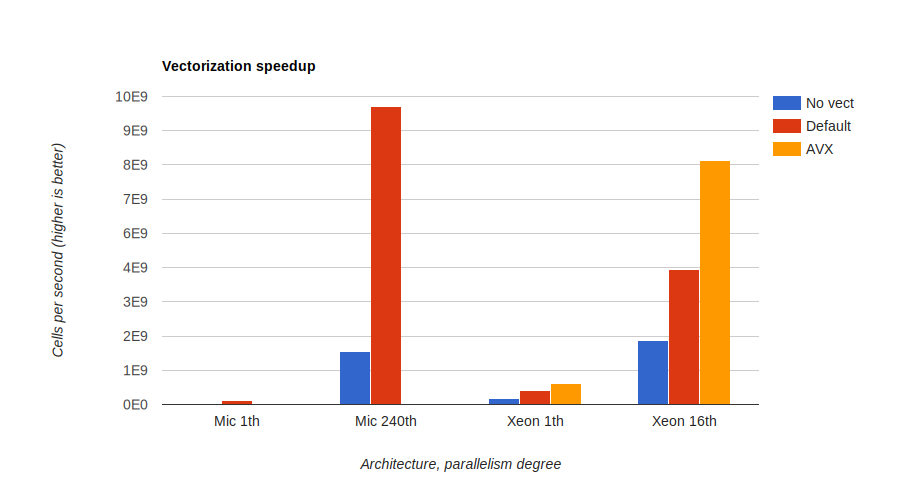
\includegraphics[width=\textwidth]{charts/vectorization-speedup.pdf}
\caption{Vectorization speedup} \label{fig:vectspeedup}
\end{figure}

% Tests:
% - sizes 4000 and 8000, 1000 iterations
% - xeon and xeonphi architectures
% - vectorization speedup
% - performance measures

% Conclusions:
% - Fastflow is easy
% - userspace spinwait is better on xeonphi
% - seq/parallel performance on xeon vs. xeonphi

\end{document}